\section{Mediciones}

\subsection{Instrumental utilizado}

Para las mediciones se utilizó un osciloscopio \textit{Tektronix MSO 70404C},
en la figura \ref{fig:osciloscopio} puede observarse el mismo. El instrumento 
posee \qty{4}{\giga\hertz} de ancho de banda analógico, y una tasa de muestreo
de \qty[per-mode=symbol]{25}{\giga\siemens\per\second} \cite{oscilloscope_datasheet}.

\subsubsection{Seguridad del instrumento}

La impedancia de entrada de entrada del instrumento es de \qty{50}{\ohm} y cumplía 
el rol de carga para el generador de pulsos. Dado el cuantioso costo del
instrumento, era fundamental garantizar que el circuito bajo ninguna condición
fuera a entregar una potencia potencialmente peligrosa para el mismo.

El osciloscopio tiene especificada una tensión de entrada máxima de $5 \ V_{RMS}$
para una resolución $\geq \ 100 \ mV/div$ y $1 \ V_{RMS}$ para una resolución
$< \ 100 \ mV/div$.

En condiciones normales de funcionamiento, la potencia disipada por la carga es
mínima, ya que es la potencia que disipa el tren de pulsos en un carga de
\qty{50}{\ohm}. \textcolor{red}{REFERENCIAR ACÁ LA SECCIÓN DONDE SE DESARROLLA
ESTA EXPRESIÓN}.

No solo es necesario analizar la disipación de potencia en condiciones normales
de funcionamiento, sino también para el caso de una falla, ya que el principal
objetivo es garantizar la integridad del instrumento en cualquier condición.

En caso de haber alguna falla con algún componente del circuito, el \textit{stub}
de salida provee una función de protección. Este componente, para señales con
una variación temporal mucho mayor al largo del mismo, actúa como una puesta a
tierra.

Entonces, la componente de continua a la salida del generador de pulsos tiene un
valor esperado de \qty{0}{\volt}, tanto para condiciones normales de 
funcionamiento como en presencia de fallas.

En cuanto a la componente alterna de la salida, su valor esperado es
extremadamente bajo, ya que únicamente señales de gran ancho de banda pueden ser
filtradas y permanecer con una amplitud considerable a la salida del 
\textit{stub}.

\begin{figure}
  \centering
    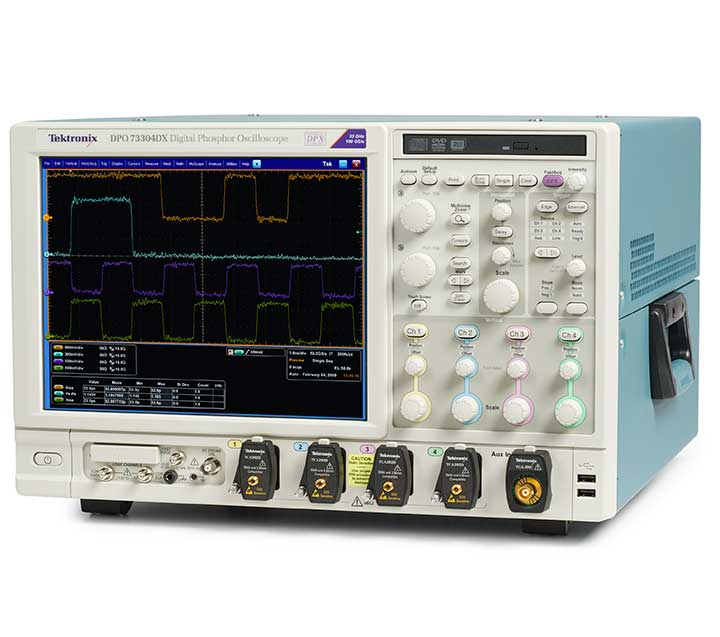
\includegraphics[width=0.5\textwidth]{images/osciloscopio.png}
    \caption{Osciloscopio \textit{Tektronix MSO 70404C}}
    \label{fig:osciloscopio}
\end{figure}

\subsection{Banco de medición}

En la figura \ref{fig:banco_medicion} puede observarse el esquema del banco de
medición. Consistió de los siguientes bloques

\begin{itemize}
    \item Placa FPGA: consistía de una placa de desarrollo \textit{Nexys 4 DDR}.
      La función de este componente era la de generar el pulso cuadrado
      unipolar, que controla la $PRF$ y el ciclo de trabajo del pulso del driver.
    \item Fuente de alimentación: provee DC para el driver. La amplitud de esta
        fuente determina la amplitud del pulso unipolar del driver.
    \item Driver: tiene tres funciones: actuar como buffer para la FPGA, de
        manera que la carga exigida sea baja, convertir la amplitud digital del
        pulso de la FPGA a la amplitud de la fuente de alimentación, y convertir
        el pulso unipolar en uno bipolar.
    \item \textit{Pulser}: el \textit{DUT}, genera los pulsos en base a la salida del driver.
    \item Osciloscopio: instrumento de medición del experimento. Actúa como
      carga con su impedancia de entrada de \qty{50}{\ohm}.
\end{itemize}

\begin{figure}
  \centering
    \includegraphics[width=0.6\textwidth]{images/banco_medicion.png}
    \caption{Banco de medición}
    \label{fig:banco_medicion}
\end{figure}

\subsubsection{Fuente de alimentación}

La fuente de alimentación era una \textit{Marconi Instruments TF2154}, en la figura 
\ref{fig:mediciones_fuente} puede observarse la misma.

Presentaba limitación de corriente regulable e indicadores para la amplitud y la
corriente entregada, lo que permitía trabajar de manera segura, dentro de los
límites de consumo obtenidos en las simulaciones anteriores.

Como fuese explicado en la sección \textcolor{red}{REFERENCIAR SECCIÓN CON CALCULOS DE POTENCIA},
la corriente máxima esperada en las condiciones de trabajo era menor a \qty{200}{\milli\ampere},
por lo que se monitoreó durante todo el experimento que la corriente entregada por la fuente
no supere este máximo teórico.

\begin{figure}
  \centering
    \includegraphics[width=0.4\textwidth]{images/mediciones_fuente.png}
    \caption{Fuente de alimentación \textit{Marconi Instruments TF2154}.}
    \label{fig:mediciones_fuente}
\end{figure}


\subsubsection{FPGA}

La \textit{FPGA} cumplía el rol de excitación del sistema. Generaba el pulso
unipolar cuadrado de entrada, que controla la $PRF$ y el ciclo de trabajo del 
pulso del driver. La \textit{FPGA} utilizada es una \textit{Artix-7} de Xilinx,
montada en una placa de desarrollo \textit{Nexys-4 DDR} de Digilent
\cite{digilent_nexys4ddr}. En la figura
\ref{fig:mediciones_fpga} puede observarse la misma. 

Las variables de ajuste del pulso unipolar eran las siguientes

\begin{itemize}
  \item Frecuencia: la frecuencia de la señal cuadrada de entrada es igual a la
    frecuencia de repetición de pulsos ($PRF$) del sistema. 
  \item Ciclo de trabajo: el ciclo de trabajo de la señal cuadrada unipolar
    determina los extremos de la señal cuadrada unipolar. A mayor ciclo de
    trabajo, valores más negativos.
\end{itemize}

Como fuera explicado anteriormente, a mayor tensión en la porción negativa del
pulso bipolar, mayor amplitud de pulso a la salida. Por lo tanto, para poder
medir las mayores amplitudes de pulso posibles era necesario para el pulso de
entrada alcanzar el mayor ciclo de trabajo posible.

El circuito programado en la FPGA consistía en un generador de cuadrada con
ciclo de trabajo variable. Mediante dos botones externos, disponibles en la
placa, se podía subir y bajar el ciclo de trabajo.

Debido a la implementación del circuito, con un contador, el paso de estas
variaciones era de un \qty{10}{\percent}.

En el anexo \ref{app:verilog} puede inspeccionarse el \textit{HDL} del circuito implementado.

\begin{figure}
  \centering
    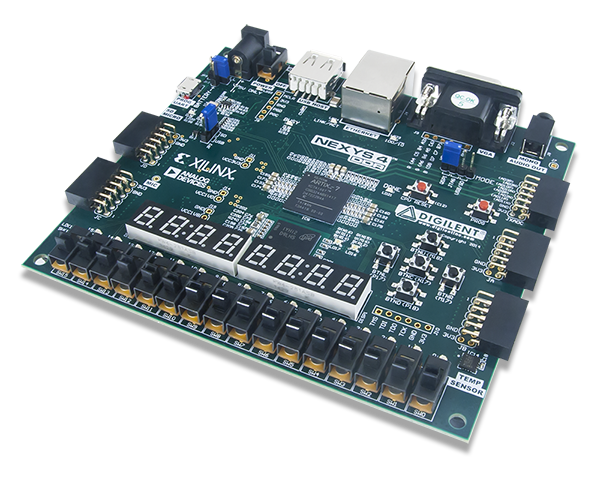
\includegraphics[width=0.4\textwidth]{images/mediciones_fpga.png}
    \caption{\textit{FPGA} utilizada}
    \label{fig:mediciones_fpga}
\end{figure}

\subsection{Mediciones realizadas}

Las mediciones consistieron en mediciones en del dominio del pulso de salida. Se
midieron tiempo de crecimiento, tiempo de decaimiento, amplitud máxima, y ancho
a medio máximo (\textit{FWHM} del inglés \textit{Full Width at Half Maximum}).

Se realizaron distintas mediciones para distintas condiciones del circuito. Se
barrió para el pulso digital de entrada, el ciclo de trabajo, y para la fuente
de alimentación distintos valores de tensión.

\begin{itemize}
    \item Para la amplitud de la fuente, se utilizaron valores de \qty{5}{\volt} y
        \qty{7}{\volt}.
        \begin{itemize}
            \item \qty{5}{\volt} por ser un valor fácilmente obtenible en los
                sistemas \textit{UWB} de referencia.
            \item \qty{7}{\volt} por ser la máxima amplitud tolerable por el circuito.
                Tensiones de alimentación mayores a estas resultan en corrientes de
                polarización mayores a las máximas admisibles dado los
                dimensionamientos de las pistas de los \textit{PCBs}.
        \end{itemize}
    \item El ciclo de trabajo se barrió entre \qty{50}{\percent} y
        \qty{70}{\percent}.
        \begin{itemize}
            \item Se tomo 50\% como límite inferior por ser un valor fácilmente
                obtenible como división de un reloj digital.
            \item Se tomo 70\% como límite superior ya que se observó que valores
                superiores a este resultaban en un pulso bipolar con amplitudes
                negativas decrecientes, y por lo tanto, amplitudes de pulso
                decrecientes.
            \item La teoría no indicaba un límite superior para el ciclo de
                trabajo. Sin embargo, este se observó en la práctica debido a no
                idealidades en el pulso de salida del driver, que no era
                perfectamente cuadrado.
        \end{itemize}
\end{itemize}

En la figura \ref{fig:sistema_medido} puede observarse el \textit{pulser} junto con el
\textit{driver} y la \textit{FPGA}.

\begin{figure}
  \centering
    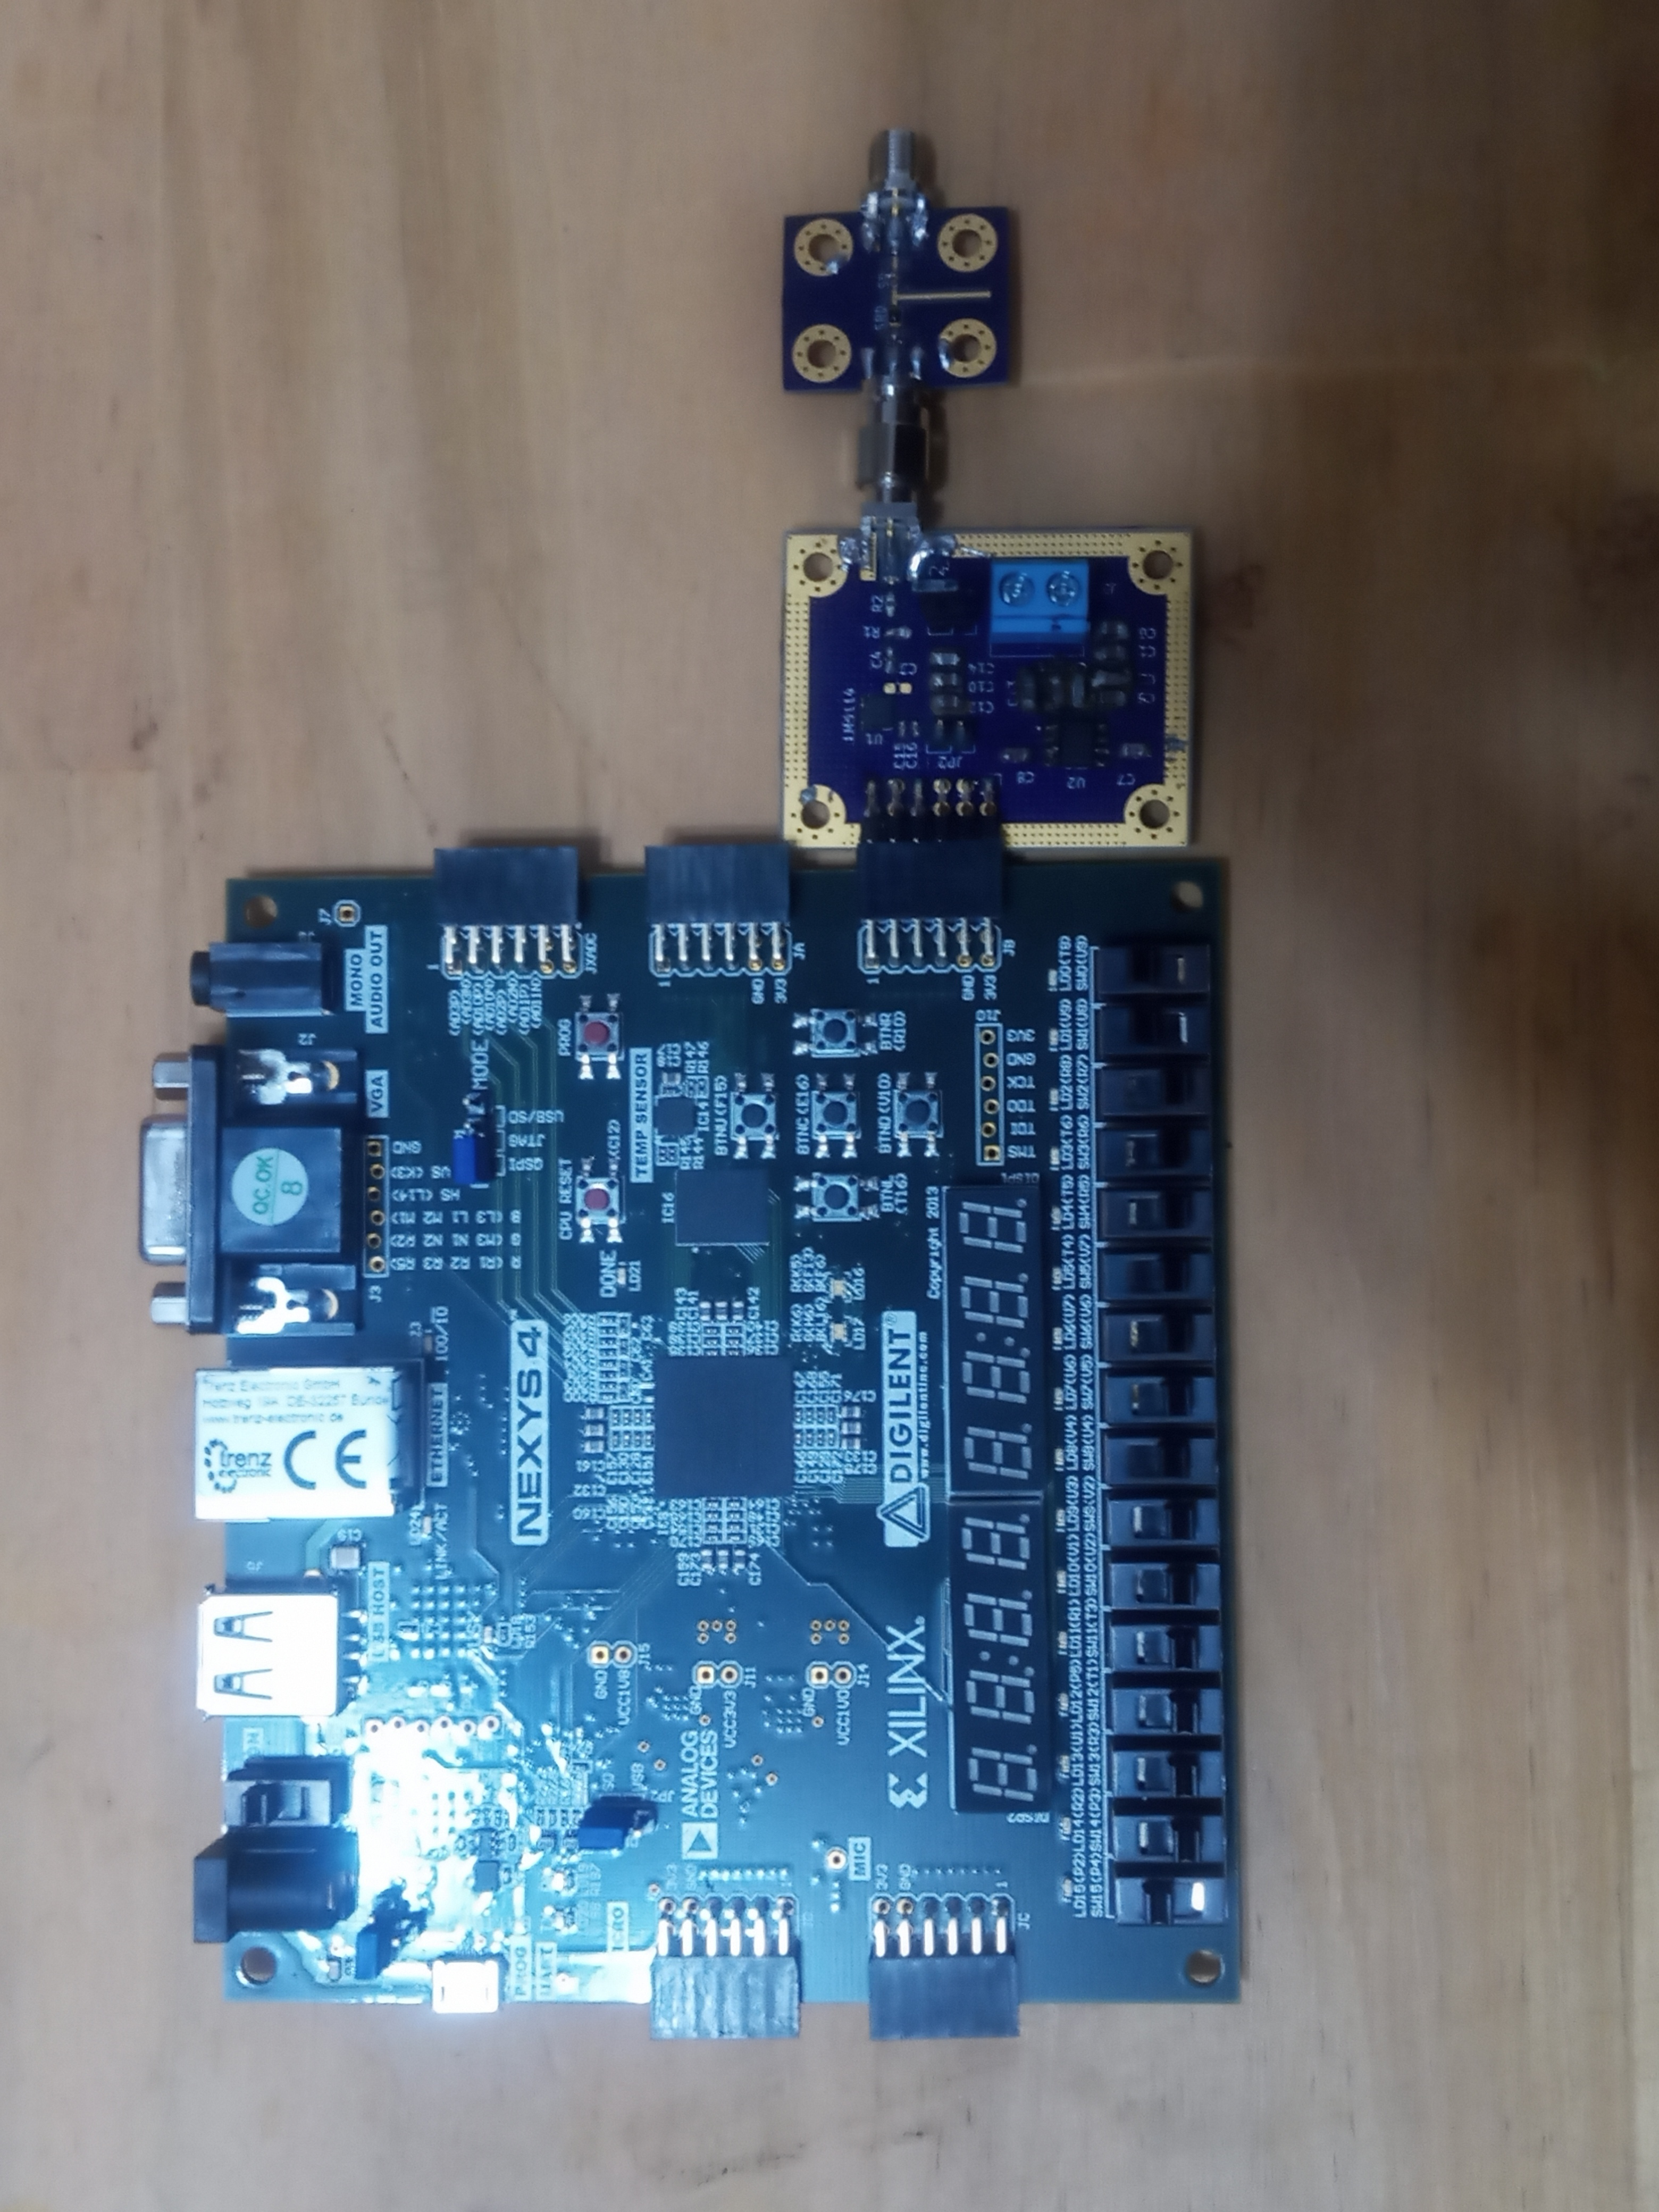
\includegraphics[width=0.4\textwidth]{images/sistema_medido.jpg}
    \caption{\textit{FPGA}, \textit{driver} y \textit{pulser}.}
    \label{fig:sistema_medido}
\end{figure}

\subsubsection{Mediciones previas}

Previo a las mediciones principales, se realizó una medición de la salida del driver,
con el objetivo de validar el pulso bipolar generado.

El motivo de esta medición previa, fue a la limitada disponibilidad del osciloscopio de
gran ancho de banda utilizado para la medición final del pulso. Esta pre-medición del pulso bipolar,
se realizó con un osciloscopio de bajo ancho de banda, ya que el objetivo era validar los niveles de
tensión del pulso, y su correcta variación con la variación del ciclo de trabajo del pulso unipolar.

En la figura \ref{fig:banco_pre_mediciones} puede observarse el banco de medición. Los resultados fueron los esperados y,
por lo tanto, no se requirió ninguna iteración sobre el diseño.

\begin{figure}
  \centering
    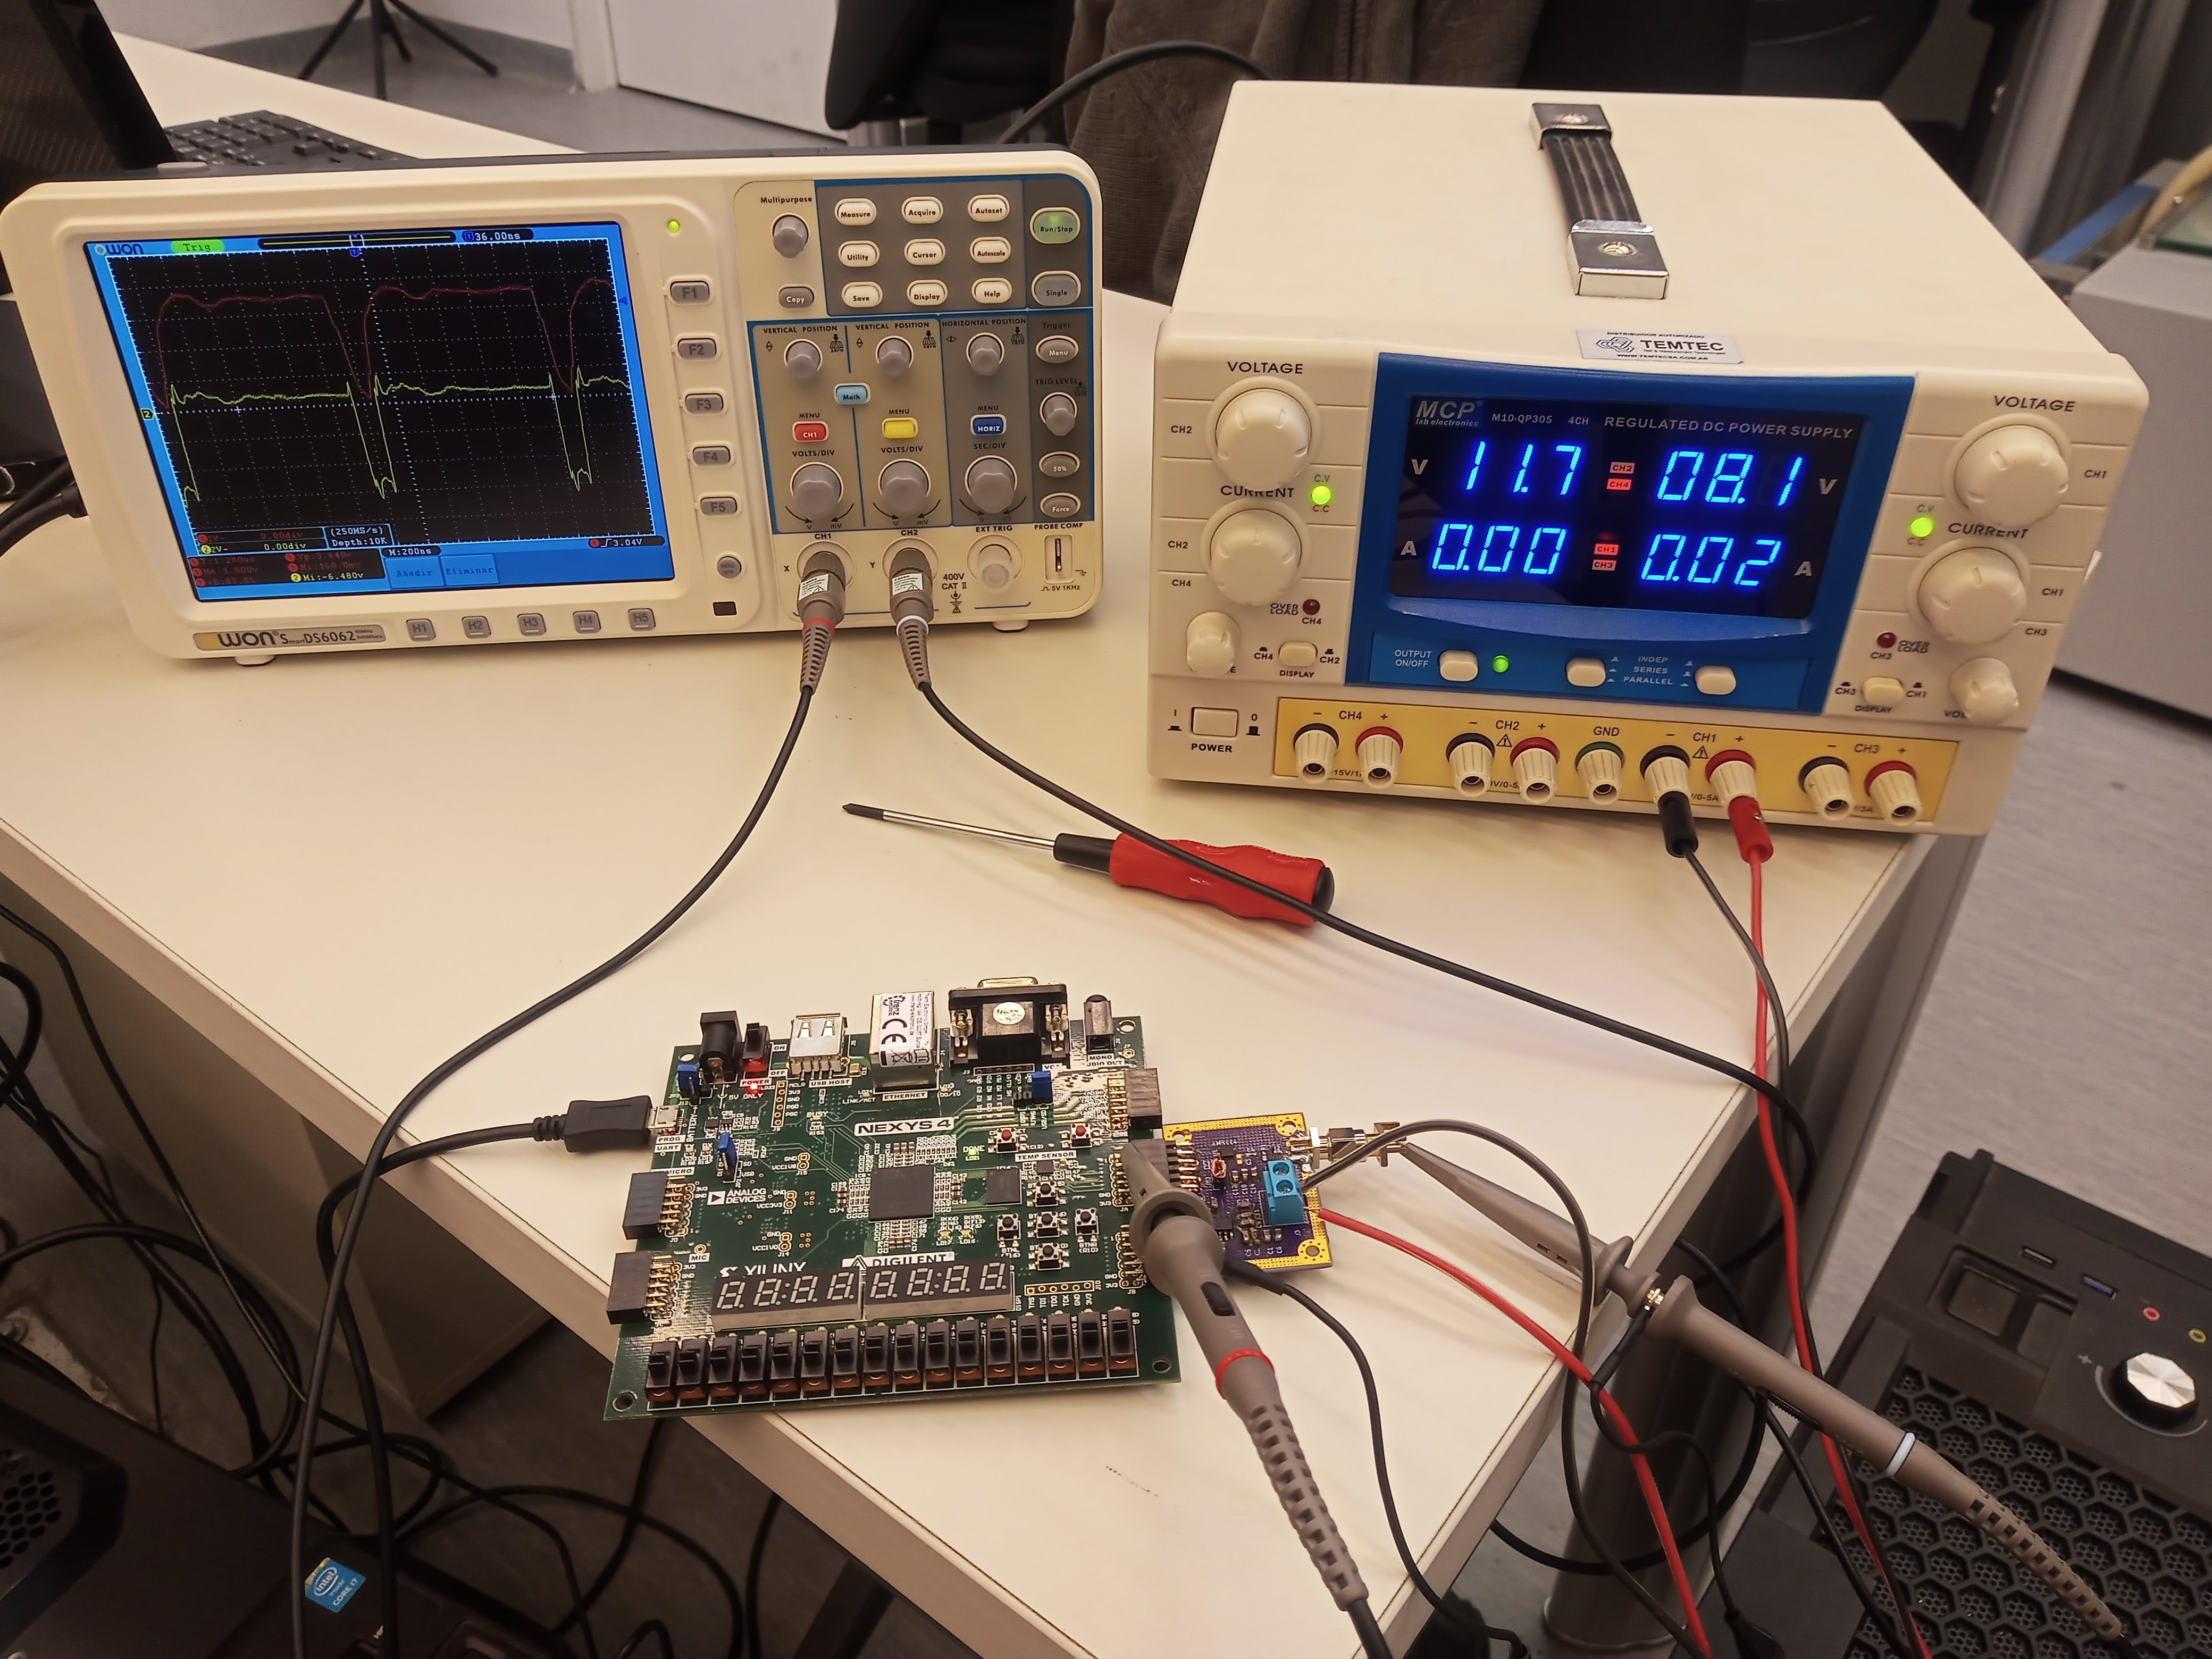
\includegraphics[width=0.4\textwidth]{images/banco_pre_mediciones.jpg}
    \caption{Banco de mediciones previas a la medición final del pulso.}
    \label{fig:banco_pre_mediciones}
\end{figure}

\subsection{Resultados}

En las figuras \ref{fig:mediciones_5v_50}, \ref{fig:mediciones_5v_70},
\ref{fig:mediciones_7v_50}, \ref{fig:mediciones_7v_60},
\ref{fig:mediciones_7v_70} pueden observarse los resultados en diversas capturas de pantalla
tomadas del osciloscopio.

Se observó en las mediciones una amplitud de pulso creciente con mayor ciclo de
trabajo y mayor amplitud de pulso, como era esperado. La menor amplitud de pulso
obtenida fue de \qty{380}{\milli\volt} para un $V_{cc}$ de \qty{5}{\volt} y un D
de \qty{50}{\percent}, y la mayor fue de \qty{1.12}{\volt} para un $V_{cc}$
de \qty{7}{\volt} y un D de \qty{70}{\percent}

En cuanto al ancho de pulso, se mantuvo aproximadamente constante en
\qty{160}{\pico\second}, al igual que los tiempos de crecimiento y
decrecimiento, que se mantuvieron constantes en \qty{90}{\pico\second}.

En la tabla \ref{tab:mediciones_resultados} pueden observarse los resultados obtenidos.

\begin{figure}
  \centering
    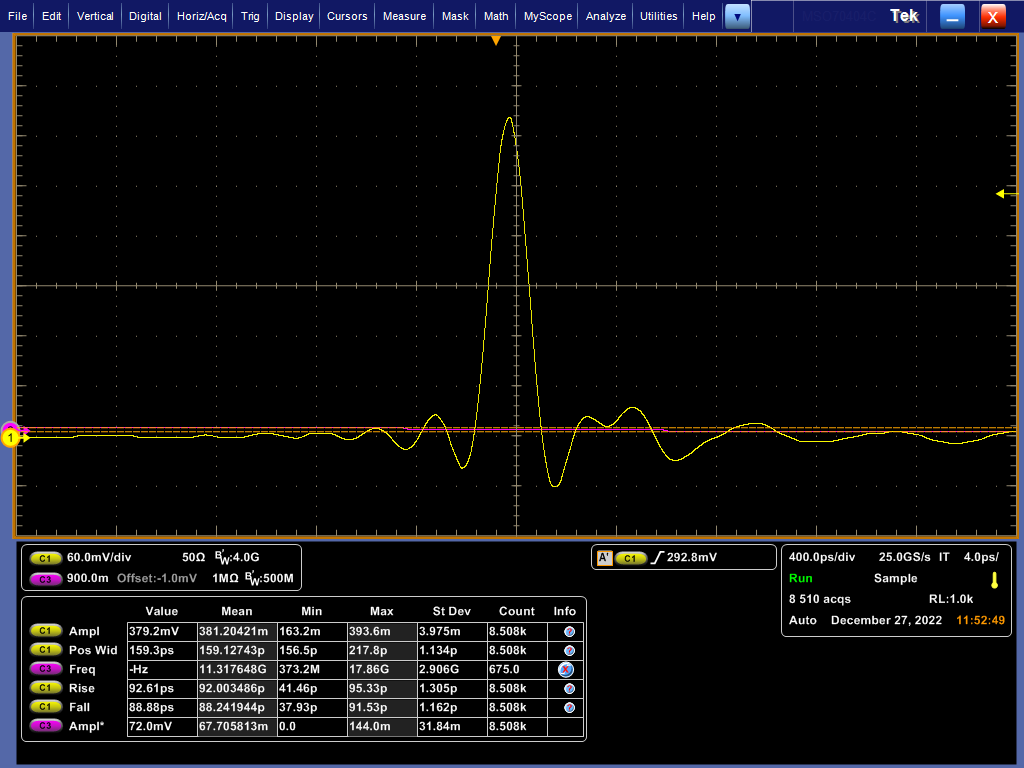
\includegraphics[width=0.6\textwidth]{images/mediciones/vcc_5v_duty_50.png}
    \caption{Salida @ $V_{cc}$ \qty{5}{\volt}, D \qty{50}{\percent} }
    \label{fig:mediciones_5v_50}
\end{figure}

\begin{figure}
  \centering
    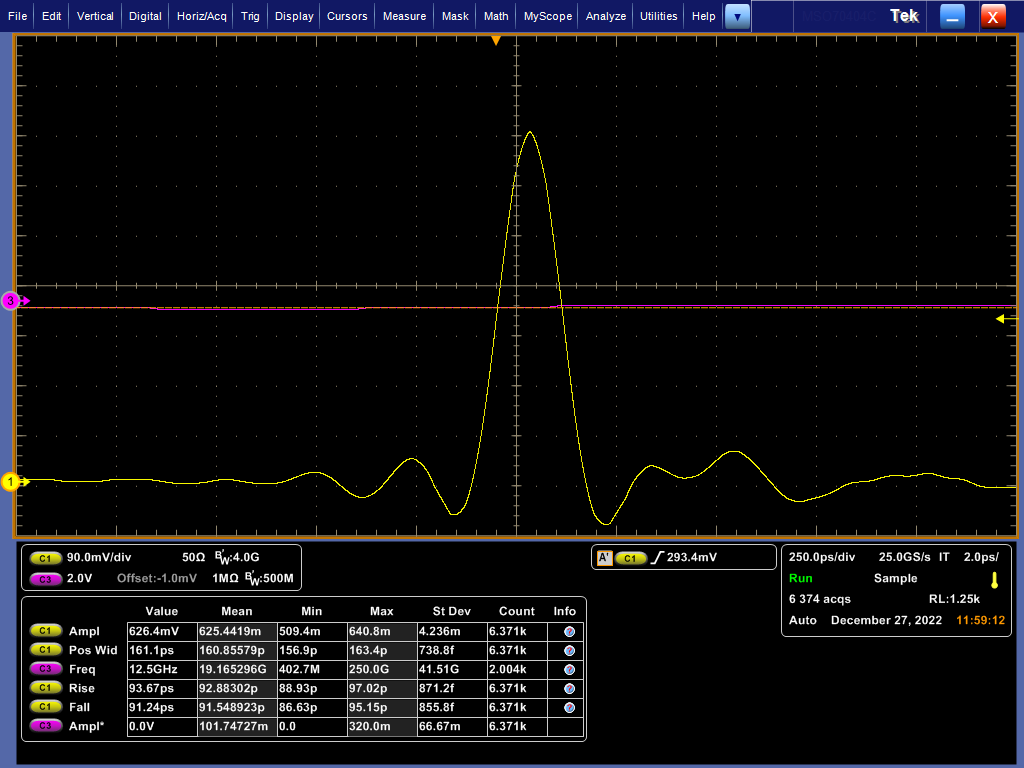
\includegraphics[width=0.6\textwidth]{images/mediciones/vcc_5v_duty_70.png}
    \caption{Salida @ $V_{cc}$ \qty{5}{\volt}, D \qty{70}{\percent} }
    \label{fig:mediciones_5v_70}
\end{figure}

\begin{figure}
  \centering
    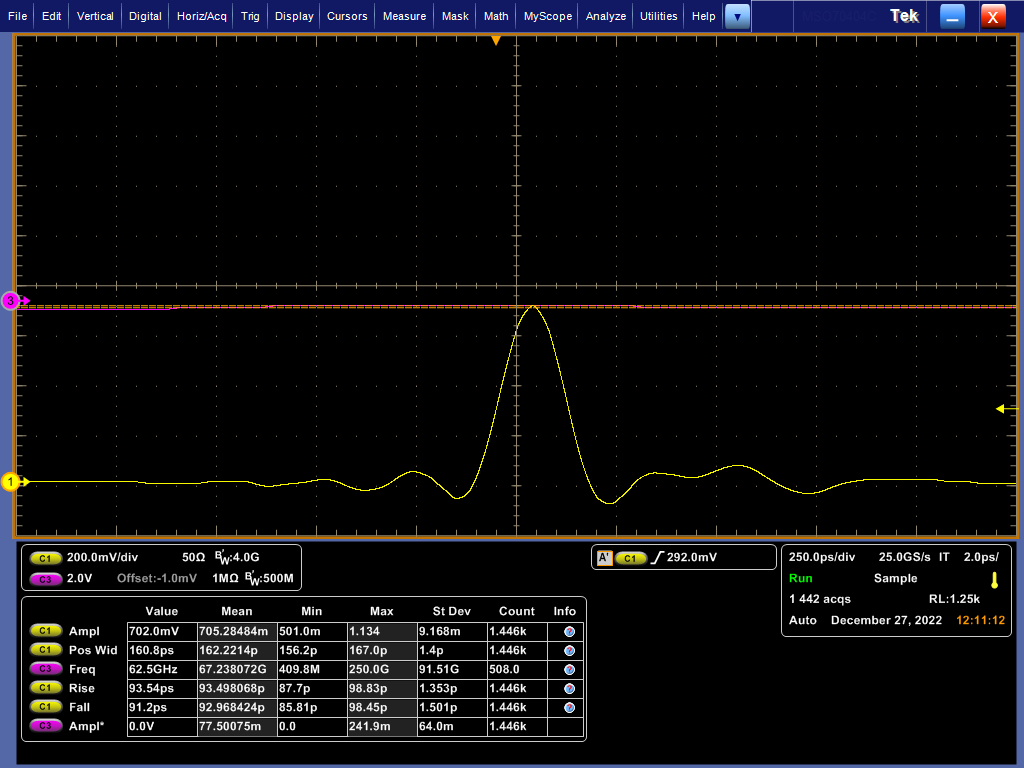
\includegraphics[width=0.6\textwidth]{images/mediciones/vcc_7v_duty_50.png}
    \caption{Salida @ $V_{cc}$ \qty{7}{\volt}, D \qty{50}{\percent} }
    \label{fig:mediciones_7v_50}
\end{figure}

\begin{figure}
  \centering
    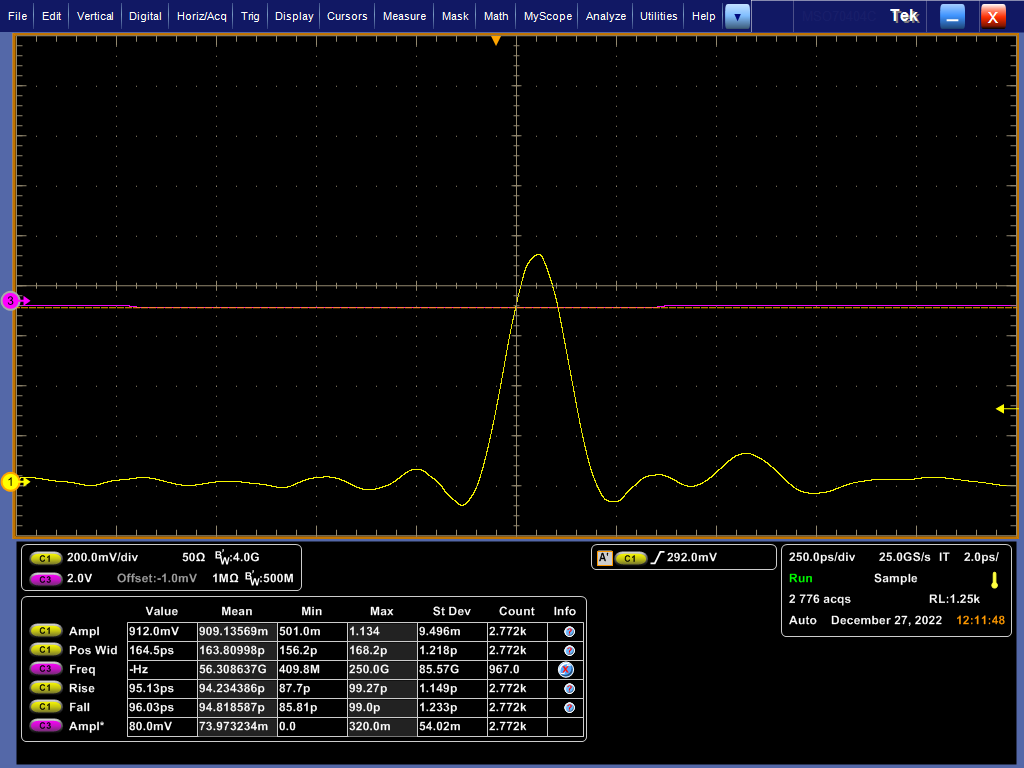
\includegraphics[width=0.6\textwidth]{images/mediciones/vcc_7v_duty_60.png}
    \caption{Salida @ $V_{cc}$ \qty{7}{\volt}, D \qty{60}{\percent} }
    \label{fig:mediciones_7v_60}
\end{figure}

\begin{figure}
  \centering
    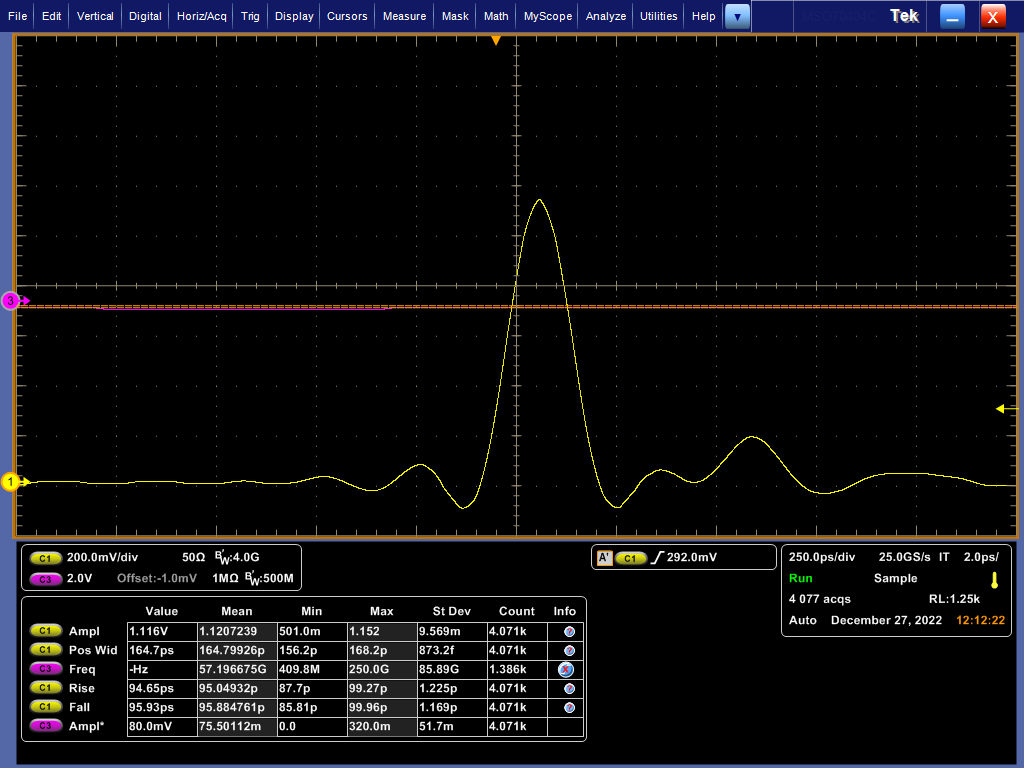
\includegraphics[width=0.6\textwidth]{images/mediciones/vcc_7v_duty_70.png}
    \caption{Salida @ $V_{cc}$ \qty{7}{\volt}, D \qty{70}{\percent} }
    \label{fig:mediciones_7v_70}
\end{figure}

\begin{table}
\centering
\begin{tabular}{ccccccc}
\hline
$V_{cc}$ [\unit{\volt}] & $D$ [\unit{\percent}] & $A$ [\unit{\volt}] &
    $FWHM$ [\unit{\pico\second}] & $\qty{3}{\dB} \ B$ [\unit{\giga\hertz}]& $t_r$
    [\unit{\pico\second}]& $t_f$ [\unit{\pico\second}]\\
\hline
5 & 50 & 0.380 & 159 & 7.5 & 93 & 88 \\
5 & 70 & 0.625 & 161 & 3.6 & 93 & 91 \\
7 & 50 & 0.702 & 162 & 4   & 93 & 93 \\
7 & 60 & 0.909 & 164 & 4   & 94 & 95 \\
7 & 70 & 1.120 & 165 & 2.8 & 95 & 96 \\
\hline
\end{tabular}
\caption{Resultados de mediciones.}
\label{tab:mediciones_resultados}
\end{table}

\subsubsection{Comparación contra simulación}

En las figuras \ref{fig:plots_5v_50} a \ref{fig:psd_7v_70} pueden observarse los resultados de las
mediciones obtenidas superpuestos con los resultados de simulación para las mismas condiciones de
trabajo (amplitud de alimentación y ciclo de trabajo).

Para las simulaciones, se toman dos resultados:

\begin{itemize}
    \item Una simulación ``ideal'', indicada como ``esquemático ideal'' en las leyendas, que se
        corresponde a una simulación sin contemplar parásitos de ningún tipo.
    \item El otro resultado corresponde a una simulación mas completa, en las leyendas ``Layout'', es
        una simulación en la que se extrajeron previamente los efectos parásitos del \textit{PCB}
        mediante una simulación electromagnética, y se incorporaron en la simulación del pulso.
\end{itemize}

Se realizan las comparaciones en el dominio del tiempo y de la frecuencia. Las comparaciones en el
dominio del tiempo consisten en la superposición del pulso medido con el simulado. Para las
comparaciones en el dominio de la frecuencia, se calculó el espectro de cada una de las formas de
onda del dominio del tiempo. Para reducir el \textit{leakage} espectral, se utilizó una ventana de
\textit{Hanning} \cite{oppenheim1999dsp}.

En el dominio del tiempo, se observa una buena coincidencia entre la amplitud de los pulsos y el
ancho. Se observa una diferencia en el \textit{ringing} de ambos.  Las simulaciones prácticamente no
presentan oscilaciones alrededor del pulso, mientras que las mediciones las presentan tanto previa
como posteriormente.  También se observa un segundo pulso de menor amplitud siguiendo al primero.

Como causa de estas discrepancias, se descarta un efecto del \textit{PCB} no modelado, ya que los
parásitos de esta estructura fueron extraídos por una simulación electromagnética, y sus efectos
contemplados en las simulaciones del \textit{layout}.

Estas  discrepancias sugieren una limitación en el modelado de alguno de los 
dispositivos, tanto el SRD como el Schottky. Las simulaciones predijeron correctamente
la amplitud y el ancho de los pulsos resultantes, pero fallaron en predecir 
el ringing y el pulso secundario.

\textcolor{red}{  
En el dominio de la frecuencia, se observa coincidencia entre los anchos de banda de los
pulsos.
EN REALIDAD NO, SE VE QUE EL PULSO 5V@50D TIENE UN ANCHO DE BANDA *MUCHO* MAYOR A 
LAS SIMULACIONES Y A LAS DEMÁS MEDICIONES.
HAY Q VER Q PASÓ AHÍ
}

\begin{figure}
  \centering
    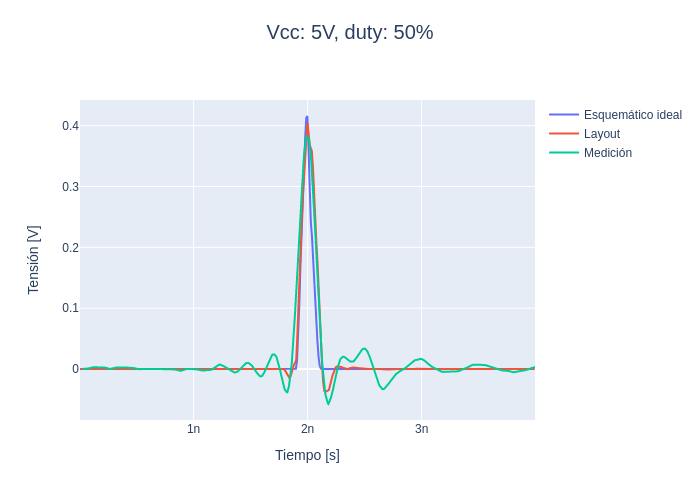
\includegraphics[width=0.6\textwidth]{images/plots/Vcc_5V_duty_50_time_domain.png}
    \caption{Pulso @ $V_{cc}$ \qty{5}{\volt}, D \qty{50}{\percent} }
    \label{fig:plots_5v_50}
\end{figure}

\begin{figure}
  \centering
    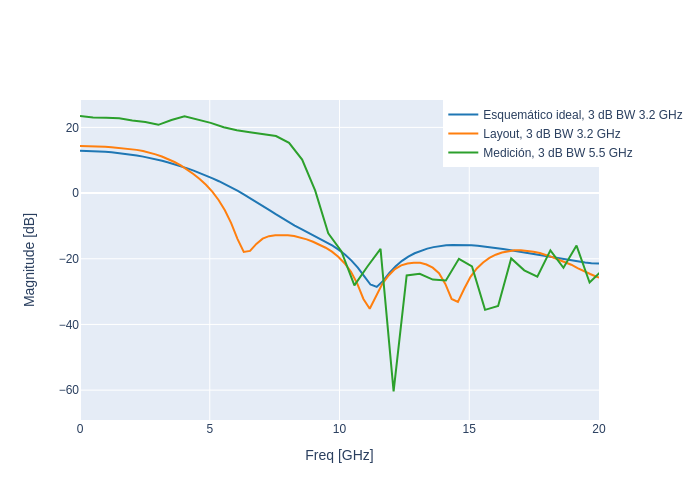
\includegraphics[width=0.6\textwidth]{images/plots/Vcc_5V_duty_50_psd.png}
    \caption{PSD @ $V_{cc}$ \qty{5}{\volt}, D \qty{50}{\percent} }
    \label{fig:psd_5v_50}
\end{figure}

\begin{figure}
  \centering
    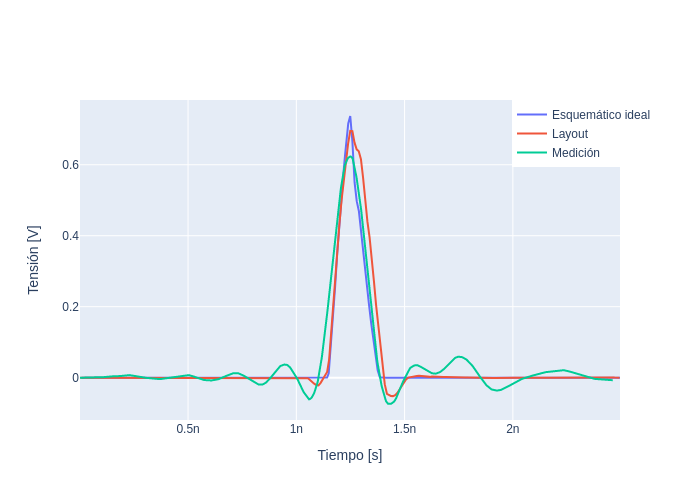
\includegraphics[width=0.6\textwidth]{images/plots/Vcc_5V_duty_70_time_domain.png}
    \caption{Pulso @ $V_{cc}$ \qty{5}{\volt}, D \qty{70}{\percent} }
    \label{fig:plots_5v_70}
\end{figure}

\begin{figure}
  \centering
    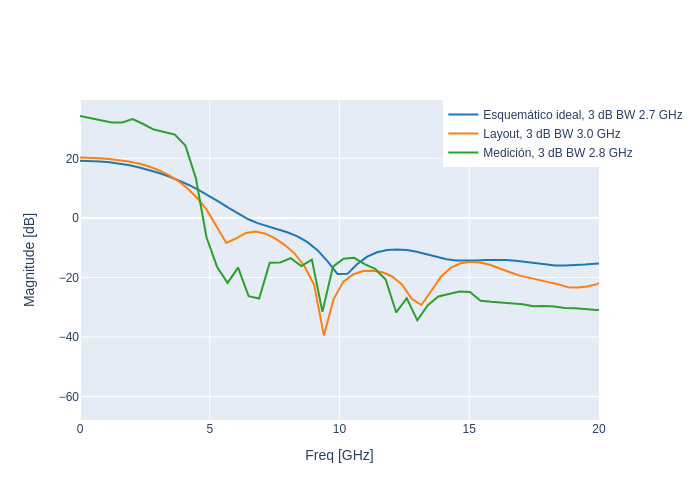
\includegraphics[width=0.6\textwidth]{images/plots/Vcc_5V_duty_70_psd.png}
    \caption{PSD @ $V_{cc}$ \qty{5}{\volt}, D \qty{70}{\percent} }
    \label{fig:psd_5v_70}
\end{figure}

\begin{figure}
  \centering
    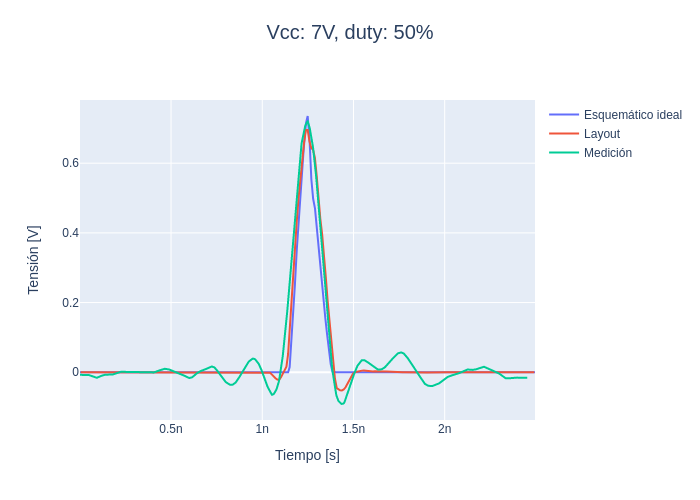
\includegraphics[width=0.6\textwidth]{images/plots/Vcc_7V_duty_50_time_domain.png}
    \caption{Pulso @ $V_{cc}$ \qty{7}{\volt}, D \qty{50}{\percent} }
    \label{fig:plots_7v_50}
\end{figure}

\begin{figure}
  \centering
    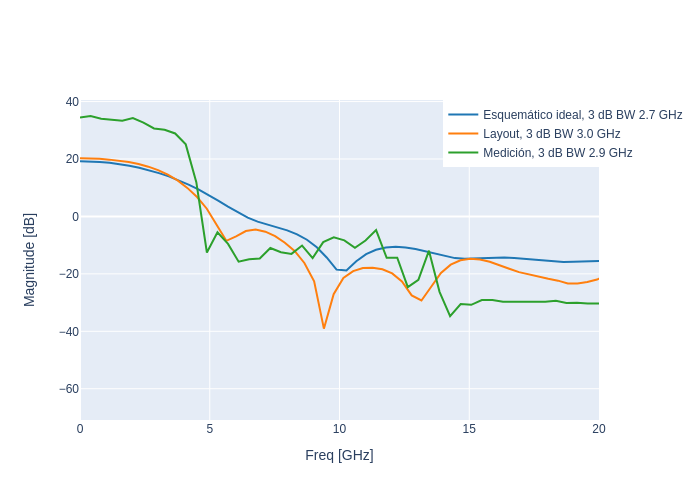
\includegraphics[width=0.6\textwidth]{images/plots/Vcc_7V_duty_50_psd.png}
    \caption{PSD @ $V_{cc}$ \qty{7}{\volt}, D \qty{50}{\percent} }
    \label{fig:psd_7v_50}
\end{figure}

\begin{figure}
  \centering
    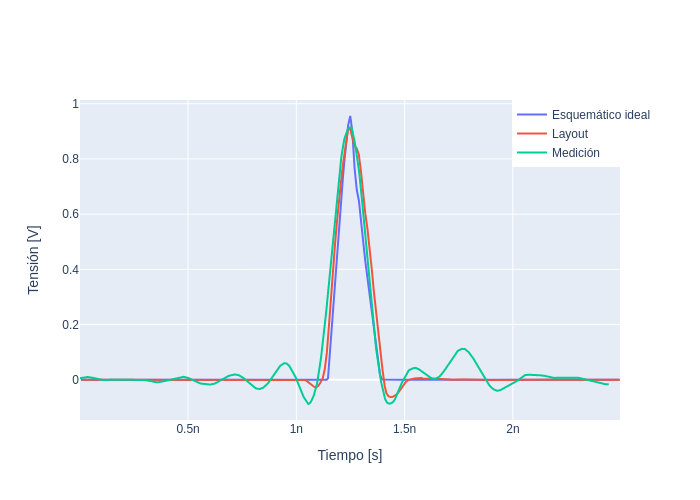
\includegraphics[width=0.6\textwidth]{images/plots/Vcc_7V_duty_60_time_domain.png}
    \caption{Pulso @ $V_{cc}$ \qty{7}{\volt}, D \qty{60}{\percent} }
    \label{fig:plots_7v_60}
\end{figure}

\begin{figure}
  \centering
    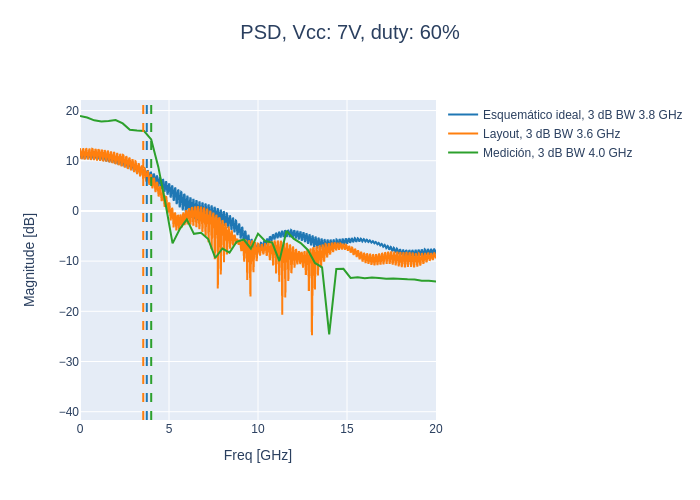
\includegraphics[width=0.6\textwidth]{images/plots/Vcc_7V_duty_60_psd.png}
    \caption{PSD @ $V_{cc}$ \qty{7}{\volt}, D \qty{60}{\percent} }
    \label{fig:psd_7v_60}
\end{figure}

\begin{figure}
  \centering
    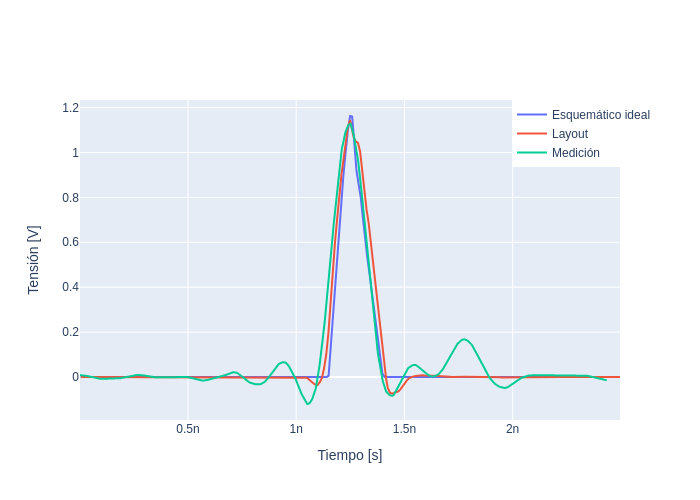
\includegraphics[width=0.6\textwidth]{images/plots/Vcc_7V_duty_70_time_domain.png}
    \caption{Pulso @ $V_{cc}$ \qty{7}{\volt}, D \qty{70}{\percent} }
    \label{fig:plots_7v_70}
\end{figure}

\begin{figure}
  \centering
    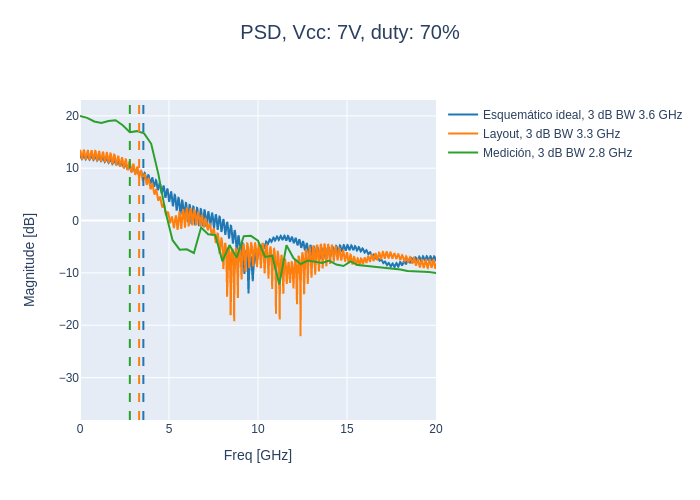
\includegraphics[width=0.6\textwidth]{images/plots/Vcc_7V_duty_70_psd.png}
    \caption{PSD @ $V_{cc}$ \qty{7}{\volt}, D \qty{70}{\percent} }
    \label{fig:psd_7v_70}
\end{figure}

\subsubsection{Comparación con resultados de la literatura}

En la tabla \ref{tab:resultados_literatura} se resumen resultados reportados para generadores de
pulsos \textit{UWB} en la literatura. En la figura \ref{fig:scatterplot_literature} se observan
los valores de amplitud y duración reportados en un gráfico de dispersión.

\begin{table}
  \begin{threeparttable}[b]
    \caption{Resultados reportados en la literatura}
    \label{tab:resultados_literatura}
    {\footnotesize
    \begin{tabular}{ccccccccc}
        \hline
        Referencia & $A$ [\unit{\volt}] & $FWHM$ [\unit{\pico\second}] &
        Bal \tnote{a} & Bias & Dispositivos & $V_{cc}$ [\unit{\volt}] & $V_{in}$ [\unit{\volt}] & $PRF$ [\unit{\mega\hertz}] \\
        \hline
        \cite{rulikowski2004} & \num{\pm 0.896}, \num{\pm 1.6} \tnote{b} & 335, 511 & Sí & Int & SRD & 5 & TTL & 50 \\
        \cite{protiva2009} & \num{-7.5} & 110 & No & Ext & SRD+3TBJ+SD & 12 & TTL & 5 \\
        \cite{kamal2014} & \num{0.8} & 170 & No & Int & SRD & 4 & 4 & 10 \\
        \cite{han2002} & \num{0.2} & 300 & No & Ext & SRD+2SD & ? & ? & 10 \\
        \cite{han2005} & \num{-6}, \num{-4} & 150 & No & Int & SRD+L & ? & 5 & 12 \\
        \cite{oloumi2018} & \num{1.27} \tnote{c} & 286 & No & Int & 2SRD+L & 10 & 10 \tnote{d} & ? \\
        \textbf{Este trabajo} & \num{1.12} & 165 & No & Int & SRD+SD & 7 & CMOS  &
        \num{10} \\
    \end{tabular}
}
   \begin{tablenotes}
     \item [a] \textit{Balanceado}.
     \item [b] la publicación presenta dos resultados, correspondientes a
       circuitos con componentes concentrados y distribuidos.
     \item [c] la publicación presenta múltiples resultados, se muestran
       los mejores.
     \item [d] la señal de entrada es senoidal.
   \end{tablenotes}
  \end{threeparttable}
\end{table}


En cuanto a los resultados reportados en este trabajo, tiene uno de los anchos de pulso más bajos,
habiendo otros trabajos que reportan el mismo o menor ancho de pulso con mayor amplitud. Otra
característica a destacar es la simplicidad del diseño implementado, tanto en cantidad de
componentes activos, como en amplitud de fuente de alimentación y pulso de entrada.

En \cite{rulikowski2004} se presenta un diseño compuesto de un solo SRD en el que se desarrolla un
pulso balanceado a la salida. Se presentan dos diseños, uno con componentes distribuidos y otro con
componentes concentrados. En ambos casos se obtienen amplitudes pico-a-pico de pulso mayores a las
de este trabajo. Es destacable que se obtienen mayores amplitudes usando una fuente de alimentación
menor, de \qty{5}{\volt}. En cuanto al ancho de pulso, ambos pulsos presentan duraciones mayores que
las de nuestro trabajo. En cuanto a la complejidad, el \textit{pulser} está implementado solamente
con 1 \textit{SRD}, y componentes distribuidos o concentrados, dependiendo de la versión, por lo que
es más simple que nuestro trabajo. El \textit{driver} presenta la misma complejidad en ambos casos,
ya que está implementado con un solo circuito integrado. Nuestro trabajo presenta más versatilidad,
ya que la amplitud de la fuente de alimentación puede variarse entre \qty{0}{\volt} y
\qty{30}{\volt}.

En \cite{protiva2009} se reporta un resultado de gran amplitud y duración de pulso menor a la de
este trabajo. El diseño presentado es de mucho mayor complejidad al de este trabajo: necesita una
alimentación de \qty{12}{\volt} y una corriente de \textit{bias} externa, y la etapa \textit{driver}
está implementada con 3 TBJs, frente a 1 solo \textit{gate driver} en nuestro trabajo.

En \cite{kamal2014} el pulso reportado es de características muy similares a las de nuestro trabajo.
La duración del pulso es prácticamente la misma, mientras que en amplitud nuestro trabajo logró un
pulso de \qty{40}{\percent} mayor amplitud. Nuestro trabajó logró para el \ŧextit{pulser} una
complejidad menor a la reportada en \cite{kamal2014}, ya que en nuestro caso omitimos la red RC y el
atenuador. En cuanto a etapa \textit{driver}, \cite{kamal2014} no presenta ninguna, en los
resultados se reporta haber utilizado como entrada al \textit{tpulser} un pulso bipolar.

En \cite{han2002} el generador presentado desarrolla pulsos monociclo, que son la primera derivada
de un pulso gaussiano. Nuestro trabajó logro una amplitud de pulso mayor y también una duración de
pulso menor. No se especifica el valor de amplitud de señal de entrada utilizado. La entrada al
circuito es bipolar, y no se incluye un \textit{driver} de adaptación de pulso. La complejidad del
generador descripto es mayor que la de este trabajo, utilizando bias externo, un diodo SRD y dos
Schottky. Sin embargo, el generador de \cite{han2002} implementa un monociclo que es una derivada de
un pulso gaussiano como el desarrollado en nuestro trabajo, por lo que es natural que la complejidad
sea mayor.

El resultado reportado en \cite{han2005} consiste en pulsos de mayor amplitud y menor duración. En
ambos casos, el pulser se encuentra acoplado por \textit{AC}, lo que vuelve más complejo el diseño.
Se presentan dos generadores, uno con línea de transmisión, y otro con un inductor, que utiliza al
SRD en paralelo. El diseño con inductor es más complejo, ya que este se encuentra en el camino del
pulso por lo que debe ser seleccionado con cuidado. En ambos casos se utiliza una red RC paralelo,
mientras que en nuestro trabajo no.

El resultado de \cite{oloumi2018} consiste en un pulso de mayor amplitud y mayor ancho al de nuestro
trabajo. La complejidad del diseño es mayor, ya que utiliza dos SRD y un inductor que se encuentra
en el camino de alta frecuencia, por lo que es costoso de seleccionar. La señal de entrada es una
senoidal, que para el contexto en el que desarrollamos nuestro generador, es más costosa de
conseguir, ya que requiere algún DAC, frente a la excitación de nuestro generador que es una señal
cuadrada, fácilmente obtenible como salida digital de una FPGA o microcontrolador.

\begin{figure}
\centering
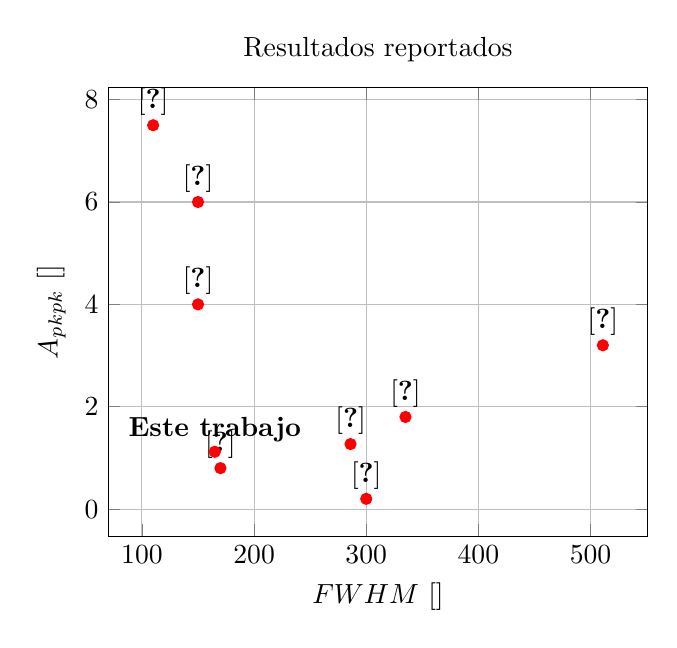
\begin{tikzpicture}
  \begin{axis}[
    xlabel={$FWHM$ [\unit{\pico\second}]},
    ylabel={$A_{pkpk}$ [\unit{\volt}]},
    title=Resultados reportados,
    grid=both
    ]
    \addplot[
        scatter/classes={a={blue}, b={red}},
        scatter, mark=*, only marks, 
        scatter src=explicit symbolic,
        nodes near coords*={\Label},
        visualization depends on={value \thisrow{label} \as \Label} %<- added value
    ] table [meta=class] {
        x   y       class   label
        511 3.2     b       {\cite{rulikowski2004}}
        335 1.8     b       {\cite{rulikowski2004}}
        110 7.5     b       {\cite{protiva2009}}
        170 0.8     b       {\cite{kamal2014}}
        300 0.2     b       {\cite{han2002}}
        150 6       b       {\cite{han2005}}
        150 4       b       {\cite{han2005}}
        286 1.27    b       {\cite{oloumi2018}}
        165 1.12    b       {\textbf{Este trabajo}}
    };

  \end{axis}
\end{tikzpicture}
  \caption{Diagrama de dispersión de resultados reportados.}
  \label{fig:scatterplot_literature}
\end{figure}
